% Página
\section{Confidencialidade}

A Confidencialidade refere-se à garantia de que as informações são acessíveis apenas por pessoas autorizadas. Em outras palavras, é a proteção contra a divulgação não autorizada de dados. Este pilar é essencial para manter a privacidade dos dados pessoais e sensíveis, como informações financeiras, médicas ou estratégicas de uma organização. Técnicas de criptografia são amplamente utilizadas para garantir a confidencialidade, assegurando que, mesmo que os dados sejam interceptados, eles não possam ser lidos ou compreendidos por indivíduos não autorizados.

\subsection{Algoritmo Assimétrico}

O algoritmo de criptografia assimétrica é uma técnica fundamental no campo da segurança e criptografia. Diferente dos algoritmos de criptografia simétrica, que utilizam a mesma chave para criptografar e descriptografar os dados, os algoritmos assimétricos usam um par de chaves: uma \textbf{chave pública(KPu)} e uma \textbf{chave privada(KPr)}. Vamos explorar o funcionamento desse algoritmo através dos personagens Alice, Bob e Eva exemplificado pela Figura \ref{fig:algoritmo_assimetrico}.

\begin{figure}[H]
	\centering
	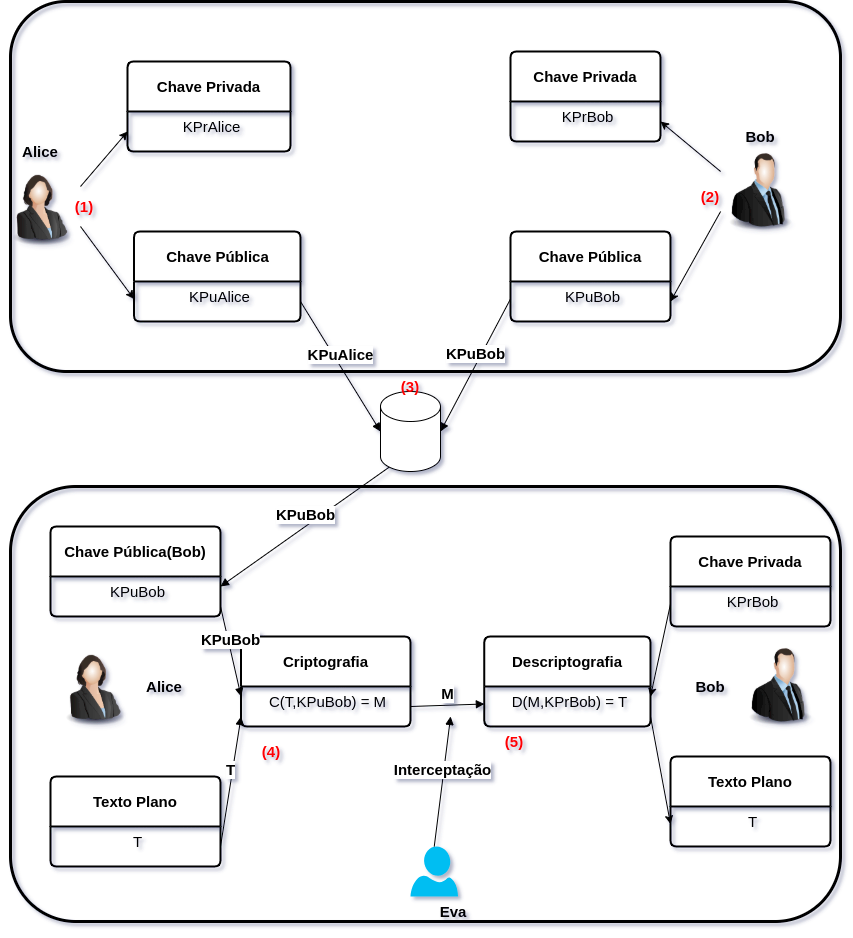
\includegraphics[scale=0.45]{algoritmo_assimetrico.png}
	\caption{Funcionamento do algoritmo de criptografia assimétrico}
	\label{fig:algoritmo_assimetrico}
\end{figure}

\pagebreak
